%% This is an example first chapter.  You should put chapter/appendix that you
%% write into a separate file, and add a line \include{yourfilename} to
%% main.tex, where `yourfilename.tex' is the name of the chapter/appendix file.
%% You can process specific files by typing their names in at the 
%% \files=
%% prompt when you run the file main.tex through LaTeX.
\chapter{Modular Sensor Fusing}
\label{chap:sensor_fusing}

In previous chapter, we learned how to represent each frame and analysed the difference between filter method and keyframe BA method for our odometry system. We also learned quaternion algebra and basic approaches for quaternion integration and derivative over the time under some general assumptions. In this chapter, we will explore the details of our sensor fusing approach, which uses so called \textit{IMU loose integration framework}~\cite{weiss2012vision}. In such a framework, system propagates states via Kalman filter (KF) based on IMU measurements, and extrasensory (\eg, camera, GPS \etc) data are used in correction step. The computational cost for Kalman-filter-styled approach is usually linear, hence \textit{IMU loose integration framework} provides a better trade-off between computational complexity and accuracy in a real-time robotic navigation system.

\section{Error-state Kalman Filter for IMU Integration}
\label{sec:ESKF_IMU}

The error-state Kalman filter (ESKF) follows the paradigm of Kalman filter, which also has prediction step and correction step. However, ESKF separates system into three different states: true state, nominal state, and error state. Nominal state processes large signal, which is integrable in a non-linear fashion, whereas error state keeps track of error and noise term, which can be integrated in a linear way. The composition of nominal state and error state, and we call it true state, which is the final guess of the system.

The ESKF has several beneficial properties when building a visual-inertial odometry:                                                                                                                                                                                                                                                                                                              
\begin{enumerate}
	\item The computation of Jacobian may be very fast, because the error state is small and all second order products are negligible. This is an important factor building a real-time system.
	\item Fusing visual data with IMU data is straightforward in Kalman filter correction step. One can utilize the tracking result to correct the IMU integration state.
	\item Large signals have been integrated into nominal states, so that we can apply the correction step in a lower rate than prediction step.
\end{enumerate}

The procedure of ESKF in this system can be explained as follows. Firstly, IMU data is integrated into nominal state via numerical integration methods, note that nominal state does not take noise terms or error terms into account, hence nominal state will accumulate errors. The error state then predict the errors and noise terms using normal extended KF paradigm, meaning it will predict the mean and covariance of the error state. In parallel a correction step is performed at a lower rate, the results of visual tracking are used to correct the error state, the error state is then injected into nominal state, which the nominal state becomes the final guess of system at that time point. The system continues until the criterion condition has been met.

We explain the ESKF for IMU integration in this section, and visual sensor as correction data in Section \ref{sec:camera_comple_data}.

%\subsection{Motivation}
%\label{subsec:ESKF_IMU_sub1}

\subsection{System Kinematics}
\label{subsec:ESKF_IMU_sub2}

We denote our true state $\vec{x}_t$ as
\begin{equation}\label{f1}
	\vec{x}_t = \vec{x}_n \oplus \vec{x}_e,
\end{equation}
where $\vec{x}_n$ is the nominal state for large signals, $\vec{x}_e$ is error state for small error/noise signal, and we have used $\oplus$ to denote a general composition step. 

We then introduce position $\vec{p}$, velocity $\vec{v}$, quaternion $\vec{q}$, accelerometer bias $\vec{a}_b$, gyroscope bias $\vec{\omega}_b$ and gravity vector $\vec{g}$ into true state, nominal state and error state respectively. The general composition step can be shown as
\begin{align}
	\vec{p}_t =& \vec{p}_n + \vec{p}_e \\
	\vec{v}_t =& \vec{v}_n + \vec{v}_e \\
	\vec{q}_t \approx& \vec{q}_n \otimes \begin{bmatrix} 1 \\ \vec{\theta}_e / 2 \end{bmatrix} \label{f2}\\
	\vec{a}_{bt} =& \vec{a}_{bn} + \vec{a}_{be} \\
	\vec{\omega}_{bt} =& \vec{\omega}_{bn} + \vec{\omega}_{be} \\ 
	\vec{g}_t =& \vec{g}_n + \vec{g}_e,
\end{align}
note that we derive Equation (\ref{f2}) by the small angle approximation (Equation (\ref{q30})). We apply angular error $\vec{\theta}_e$ instead of quaternion error in error state following classical approaches.

We then construct kinematic equations for true state, which are
\begin{align}
	\label{f18}
	\dot{\vec{p}_t} =& \vec{v}_t \\
	\dot{\vec{v}_t} =& \mR_t(\vec{a}_m - \vec{a}_{bt} - \vec{a}_n) + \vec{g}_t\\
	\dot{\vec{q}_t} =& \frac{1}{2}\vec{q}_t \otimes (\vec{\omega}_m - \vec{\omega}_{bt} - \vec{\omega}_n) \\
	\dot{\vec{a}_{bt}} =& \vec{a}_w \\
	\dot{\vec{\omega}_{bt}} =& \vec{\omega}_{w} \\ 
	\label{f19}
	\dot{\vec{g}_t} =& 0,
\end{align}
where $\vec{a}_m$ and $\vec{\omega}_m$ are the measurements from accelerometer and gyroscope respectively within \textbf{local frame}, $\vec{a}_n$ and $\vec{\omega}_n$ are noises with those measurements, $\vec{a}_w$ and $\vec{\omega}_w$ are white Gaussian noise together with accelerometer and gyroscope bias, and $\mR_t$ is the rotation matrix corresponding to true state quaternion, \ie, $\mR_t \triangleq \mR_t\{ \vec{q} \}$ regarding to Equation (\ref{q25}). We use similar notations in nominal state and error state. 

We obtain kinematic equations for nominal state by cutting off all small signals, which leads to
\begin{align}
	\label{f12}
	\dot{\vec{p}_n} =& \vec{v}_n \\
	\label{f11}
	\dot{\vec{v}_n} =& \mR_n(\vec{a}_m - \vec{a}_{bt}) + \vec{g}_n\\
	\dot{\vec{q}_n} =& \frac{1}{2}\vec{q}_n \otimes (\vec{\omega}_m - \vec{\omega}_{bn})\\
	\dot{\vec{a}_{bn}} =& 0 \\
	\dot{\vec{\omega}_{bn}} =& 0 \\ 
	\label{f13}
	\dot{\vec{g}_n} =& 0,
\end{align}
and the error state with small signals is
\begin{align}
	\label{f3}
	\dot{\vec{p}_e} =& \vec{v}_e \\
	\label{f4}
	\dot{\vec{v}_e} =& \mR_n \left[ \vec{a}_m - \vec{a}_{bn} \right]_{\times} -  \mR_n\vec{a}_{be} + \vec{g}_e - \mR_n\vec{a}_n\\
	\label{f5}
	\dot{\vec{\theta}_e} =& \left[ \vec{\omega}_m - \vec{\omega}_{bn} \right]_{\times} - \vec{\omega}_{be} - \vec{\omega}_{n}\\
	\label{f6}
	\dot{\vec{a}_{be}} =& \vec{a}_w \\
	\label{f7}
	\dot{\vec{\omega}_{be}} =& \vec{\omega}_{w} \\ 
	\label{f8}
	\dot{\vec{g}_e} =& 0. 
\end{align}
It is trivial to derive Equation (\ref{f3}, \ref{f6}, \ref{f7}, \ref{f8}), see Appendix \ref{chap:appendix1} for derivation of Equation (\ref{f4} and \ref{f5}).

\subsection{State Time-integration and Error-state Jacobian}
\label{subsec:ESKF_IMU_sub3}

We propose time-integration equations between any two time stamp $t_n$ and $t_{n+1}$ where we measure the time difference $\Delta{t}$ as $\Delta{t} = t_{n+1} - t_{n}$. In order to simplify our notations, we denote last state parameters as $\vec{x}$, and denote current state parameters as $\vec{x}^{\prime}$, where current state is measured at time stamp $t_{n}$, and last state is measured at $t_{n-1}$. Same notations are set for error state. Therefore, time-integration equations for nominal state for one updating are
\begin{align}
	\vec{p}_n^{\prime} =& \vec{p}_n + \vec{v}_n\Delta{t} + \frac{1}{2}(\mR_n(\vec{a}_m - \vec{a}_{bt}) + \vec{g}_n)\Delta{t}^2 \\
	\vec{v}_n^{\prime} =& \vec{v}_n + (\mR_n(\vec{a}_m - \vec{a}_{bt}) + \vec{g}_n)\Delta{t}\\
	\label{f9}
	\vec{q}_n^{\prime} =& \vec{q}_n \otimes \vec{q}\{(\vec{\omega}_m - \vec{\omega}_{bn})\Delta{t}\}\\
	\vec{a}_{bn}^{\prime} =& \vec{a}_{bn} \\
	\vec{\omega}_{bn}^{\prime} =& \vec{\omega}_{bn} \\ 
	\vec{g}_n^{\prime} =& \vec{g}_n.
\end{align}
We use \textbf{\textit{Zeroth order forward integration}} explained in Section \ref{sec:timei_on_quat} to integrate our state over time, this is also called Euler method in Runge-Kutta numerical integration methods (see Appendix \ref{sec:runge_kutta}).

We integrate our error state in the same manner, except we have truncated second-order signal out. We obtain the integration equations for error state by
\begin{align}
	\vec{p}_e^{\prime} =& \vec{p}_e + \vec{v}_e \Delta{t}\\
	\vec{v}_e^{\prime} =& \vec{v}_e + (\mR_n \left[ \vec{a}_m - \vec{a}_{bn} \right]_{\times} -  \mR_n\vec{a}_{be} + \vec{g}_e)\Delta{t} + \vec{v}_i\\
	\label{f10}
	\vec{\theta}_e^{\prime} =& (\mR_n^T \{ \vec{\omega}_m - \vec{\omega}_{bn} \} \vec{\theta}_e - \vec{\omega}_{be})\Delta{t} + \vec{\theta}_{i}\\
	\vec{a}_{be}^{\prime} =& \vec{a}_{be} + \vec{a}_i\\
	\vec{\omega}_{be}^{\prime} =& \vec{\omega}_{be} + \vec{\omega}_i\\ 
	\vec{g}_e^{\prime} =& \vec{g}_e,
\end{align}
where $\vec{v}_i$, $\vec{\theta}_{i}$, $\vec{a}_i$, and $\vec{\omega}_i$ are random impulses for velocity, angular error, accelerometer bias and gyroscope. Those impulses can be modelled by Gaussian process. We derive Equation (\ref{f10}) by close-formed integration methods described in Appendix \ref{sec:close_integration}.

We then provide the Jacobian of error state $\mJ_{x_e}$ for ESKF prediction step usage
\begin{equation}\label{f14}
	\mJ_{e^\prime e} = \frac{\partial{\vec{x}_e^{\prime}}}{\partial{\vec{x}_e }} = \begin{bmatrix}
	\ones & \ones\Delta{t} & 0 & 0 & 0 & 0 \\
	0 & \ones & \mR_n \left[ \vec{a}_m - \vec{a}_{bn} \right]_{\times}\Delta{t} & \mR_n\Delta{t} & 0 & \ones\Delta{t} \\
	0 & 0 & \mR_n^T \{ \vec{\omega}_m - \vec{\omega}_{bn} \}\Delta{t} & 0 & -\ones\Delta{t} & 0 \\
	0 & 0 & 0 & \ones & 0 & 0 \\
	0 & 0 & 0 & 0 & \ones & 0 \\
	0 & 0 & 0 & 0 & 0 & \ones \\
	\end{bmatrix}.
\end{equation}

Note that partial derivative between true state $\vec{x}_t$ and $\vec{x}_e$ is not identity because we use different parameters to represent orientations, \eg quaternion in true state, angular error in error state. We then give the Jacobian of true state with respect to error state with
\begin{equation}\label{f15}
	\mJ_{t e} = \frac{\partial{\vec{x}_t}}{\partial{\vec{x}_e }} = \begin{bmatrix}
	\ones & 0 & 0 & 0 & 0 & 0 \\
	0 & \ones &0 & 0 & 0 & 0 \\
	0 & 0 & \frac{\partial{\vec{q}_t}}{\partial{\vec{\theta}_e }} & 0 & 0 & 0 \\
	0 & 0 & 0 & \ones & 0 & 0 \\
	0 & 0 & 0 & 0 & \ones & 0 \\
	0 & 0 & 0 & 0 & 0 & \ones \\
	\end{bmatrix}.
\end{equation}
By Equation (\ref{q5}), we have
\begin{align}\label{f16}
	\frac{\partial{\vec{q}_t}}{\partial{\vec{\theta}_e }} &= \frac{1}{2}Q^+(\vec{q})\begin{bmatrix}
	0 & 0 & 0 \\
	1 & 0 & 0 \\
	0 & 1 & 0 \\
	0 & 0 & 1 \\
	\end{bmatrix} \\
	&= \frac{1}{2}\begin{bmatrix}
	-q_x & -q_y & -q_z \\
	q_w & -q_x & q_y \\
	q_z & q_w & -q_x \\
	-q_y & q_x & q_w \\
	\end{bmatrix}. 
\end{align}

\subsection{State Propagation}
\label{subsec:ESKF_IMU_sub4}

Initially, nominal state $\vec{x}_n$ has been set to an initial guess based on the prior knowledge, and there is no error at start, \ie, error state is set to zero. We assume error state $\vec{x}_e$ as a normal distribution, \ie, $\vec{x}_e \sim \mathcal{N}(\hat{\vec{x}_e}, \mSigma)$, where $\mSigma$ denotes the covariance matrix for error state, which helps us to track the uncertainty of error state. Note that $\mSigma$ is initialized to a very small diagonal matrix.

At the certain round, we first obtain the measurements from accelerator and gyroscope, and compute a new nominal state estimation $\hat{\vec{x}_n^\prime}$ from Equation (\ref{f12}) to (\ref{f13}). We then compute error state Jacobian $\mJ_{e^\prime e}^\prime$ by Equation(\ref{f14}), then update the error state and covariance matrix of current error state by
\begin{align} \label{f22}
\hat{\vec{x}_e^\prime} &= \mJ_{e^\prime e}^\prime\hat{\vec{x}_e} \\
\mSigma^\prime &= \mJ_{e^\prime e}^\prime \mSigma (\mJ_{e^\prime e}^\prime)^T,
\end{align}
which is called \textit{prediction step} in ESKF. We omit prime symbol in the next step, \ie current state $\vec{x}$ is replaced by $\vec{x}^\prime$.

We then assume correction measurement $\vec{y}$ from extrasensory data is a non-linear function with additional white Gaussian noise $w \sim \mathcal{N}(0, \mW)$ of our true state, \ie,
\begin{equation}\label{f17}
	\vec{y} = h(\vec{x}_t) + w,
\end{equation}
and the \textit{correction step} of ESKF are as follows
\begin{align}\label{f30}
	\mK &= \mSigma\mH^T(\mH\mSigma\mH^T+\mW)^{-1} \\
	\hat{\vec{x}_e^\prime} &= \mK (\vec{y} - h(\hat{\vec{x}_t})) \\
	\mSigma^\prime &= (\ones - \mK\mH)\mSigma,
\end{align}
where $\mH$ is the Jacobian matrix of measurement function $h(\cdot)$ with respect to error state $\vec{x}_e$ (see Section \ref{subsec:camera_comple_data_sub2}). Note the estimation of true state here is the nominal state since we have not observed the mean of error state. The true state is estimated by Equation (\ref{f1}) and Equation (\ref{f18}) to (\ref{f19}). Depending on the output frequency of extra sensor, \textit{correction step} often happens on a lower rate than \textit{prediction step}. As always, we omit prime symbol in next few steps as state has been refreshed.  

Before the system enters into the next round, we reset error state to initial state, \ie, $\hat{\vec{x}_e} = 0$ in our case. We update covariance matrix $\mSigma$ by
\begin{equation}\label{f20}
	\mSigma^\prime = \mJ_{ge} \mSigma (\mJ_{ge})^T,
\end{equation}
where $\mJ_{ge}$ is Jacobian matrix of updated error state with respect to old error state. $\mJ_{ge}$ is given by
\begin{equation}\label{f21}
	\mJ_{ge} \triangleq \dfrac{\partial{\vec{x}_e^\prime}}{\partial{\vec{x}_e}} = \begin{bmatrix}
	\ones_6 & 0 & 0 \\
	0 & \ones - \left[ \frac{1}{2} \hat{\vec{\theta}_e} \right]_\times & 0 \\
	0 & 0 & \ones_9 \\
	\end{bmatrix},
\end{equation}
where we use $\vec{x}^\prime$ to denote the new state after resetting error state. The Jacobian is identical on all diagonal blocks except angular error term for the assumption we have made in Equation (\ref{q30}). We derive the $\mJ_{ge}$ by two observations, first the true state will not be able to change during the reset of error state; second, the new nominal state is obtained by injecting old error state mean from old nominal state, which the above observation can be transformed into following equations
\begin{align}
	\label{f31}
	\vec{x}_n^\prime \oplus \vec{x}_e^\prime =& \vec{x}_n \oplus \vec{x}_e \\
	\label{f32}
	\vec{x}_n^\prime =& \vec{x}_n \oplus \hat{\vec{x}_e}.
\end{align}
Putting Equation (\ref{f32}) into Equation (\ref{f31}), we have
\begin{equation}
	\vec{q}_e^\prime = (\vec{q}_n \otimes \hat{\vec{q}_e})^* \otimes \vec{q}_n \otimes \vec{q}_e = Q^+(\hat{\vec{q}_e})^*\vec{q}_e.
\end{equation}
By using small angle approximation (Equation (\ref{q5})) and throwing second order term, we can obtain 
\begin{equation}
	\vec{\theta}_e^\prime = -\hat{(\vec{\theta}_e} + (\ones - \left[ \frac{1}{2} \hat{\vec{\theta}_e} \right]_\times)\vec{\theta}_e.
\end{equation}
After derivation of old angular term from both sides, we get 
\begin{equation}
	\dfrac{\partial{\vec{\theta}_e^\prime}}{\partial{\vec{\theta}_e}} = \ones - \left[ \frac{1}{2} \hat{\vec{\theta}_e} \right]_\times,
\end{equation}
which is precisely the term in Equation (\ref{f21}).
\section{Camera as Complementary Sensory Data}
\label{sec:camera_comple_data}

As we discussed in Section \ref{sec:ESKF_IMU}, we need extrasensory data in ESKF \textit{correction step}, and we modelled this sensor as a non-linear measurement of true state $\vec{x}_t$ plus a white Gaussian noise as shown in Equation (\ref{f17}). This sensor in our case should satisfy the following conditions:
\begin{itemize}
\item {This sensor should carry rich information as we need to obtain accurate camera pose estimation from it.}
\item {This sensor, unlike GPS, should work both inside and outside environment as our system is designed for mobile robots.}
\item {This sensor should be light-weight, low-expense and better easy to handle as this is the general requirements for mobile robots.}
\end{itemize}
which lead to our choice --- camera. It is worthy to note that though we treat data in correction step as a black box, it is also possible to choose a multiple sensory platform. However on the one hand, we choose camera not only it satisfies all the above conditions, but also the camera as most commonly-used sensor has been well-investigated and well-understand, which could help us to find multiple possible approaches to solve our problem, \eg, camera pose estimation in our case; on the other hand, multiple extra sensors (\ie, camera+GPS) probably meet some issues such as synchronizing between multiple sensory platforms. Therefore we choose camera as complementary data in this work.

\subsection{Introduction to Monocular Visual Odometry}
\label{subsec:camera_comple_data_sub1}

Visual odometry estimates the camera pose, and it can provide the measurements (\eg, global translation and rotation) we need in ESKF prediction step as the transformation between camera and IMU has been pre-calibrated. We here briefly introduce different types of visual odometry system. There are stereo-based odometry \cite{mei2009constant}, depth-camera odometry \cite{newcombe2011kinectfusion}, however considering we only use single camera in this work, we mainly introduce monocular visual odometry.

A monocular odometry usually works as follows. Initially, the system obtains the first guess of camera's pose by \textit{Homography} \cite{fischler1981random} between two images. After a new image is acquired, the system then tries to find the correspondences among common \textit{landmarks}, where a landmark is defined as the most distinctive object in the real world. Depending on the types of correspondences, we have
\begin{itemize}
\item {\textbf{Feature-based methods} As proposed in \cite{davison2007monoslam, eade2007monocular, klein2007parallel, mur2015orb}, feature-based methods use image features to denote these correspondences, \eg, points are the same if the features corresponding to it are same. The system then reprojects similar points from the last image to the current one using estimated camera pose transformation, errors between points in the current visual frame is called reprojection error.}
\item {\textbf{Direct methods} As proposed in \cite{engel2014lsd}, it uses image intensity (\eg, photometric error) to find such correspondences.}
\item {\textbf{Semi-direct methods} As shown in \cite{forster2014svo}, it uses combinations of image features and image intensities to find correspondences.}
\end{itemize}
After the connections of points  between two images has been established, camera pose is estimated by minimizing the re-projection error or image intensity error.

Building a map based on such odometry is straightforward. A point is recognized as a part of landmark if it has been frequently tracked, and then will be inserted into the map as a recognized "map point"; a map is then constructed by such map points, and normally a batch processing (\eg, bundle adjustment) is used for optimizing the map during mapping process. However, such a technique can also be used for improving the pose estimation quality as we introduced in Section \ref{subsec:camera_comple_data_sub3}.

\subsection{Self-adapt Map Scale}
\label{subsec:camera_comple_data_sub2}

Estimation of camera pose from monocular visual odometry (VO) usually is a good compensation to ESKF IMU integration since global translation is unobservable to IMU integration. Since camera is an angle-sensor, it is impossible to obtain the scale of map \cite{forster2014svo}, \ie, global translation from monocular VO has been scaled up/down with real world scale. Researchers have estimated map scale factor by aligning the first few frames with ground-truth data \cite{forster2014svo}, or initialize map scale by a standard object (\eg, a A4 paer) \cite{davison2007monoslam}, and it is still likely to accumulate scale drift with time goes on. In our framework, since IMU measures under a real world scale, we can propagate the map scale in our ESKF framework by introducing a scale factor in our state. 

We first add the scale factor $\vec{\lambda}$ which contains a 3-vector to represent the scalability with x-axis, y-axis, and z-axis respectively. Now our true state, nominal state, and error state have been changed into
\begin{align}
	\vec{x}_t &= \left[ \vec{p}_t \ \vec{v}_t \ \vec{q}_t \ \vec{a}_{bt} \ \vec{\omega}_{bt} \ \vec{g}_{t} \ \vec{\lambda}_{t} \right]^T \\
	\vec{x}_n &= \left[ \vec{p}_n \ \vec{v}_n \ \vec{q}_n \ \vec{a}_{bn} \ \vec{\omega}_{bn} \ \vec{g}_{n} \ \vec{\lambda}_{n} \right]^T \\
	\vec{x}_e &= \left[ \vec{p}_e \ \vec{v}_e \ \vec{\theta}_e \ \vec{a}_{be} \ \vec{\omega}_{be} \ \vec{g}_{e} \ \vec{\lambda}_{e} \right]^T .
\end{align}
The derivative with $\vec{\lambda}$ with respect to time is easily derived since we assume the scale factor is independent with time, therefore we have
\begin{align}
	\dot{\vec{\lambda}_t} &= 0 \\
	\dot{\vec{\lambda}_n} &= 0 \\
	\dot{\vec{\lambda}_e} &= 0.
\end{align}
It is trivial to make corresponding changes to system kinematic equations (\eg, Equation \ref{f12} to \ref{f18}) and the error state Jacobian (\eg, Equation \ref{f15} and \ref{f16}). The measurement function $h(\cdot)$ of estimated true state $\dot{\vec{x}_t}$ can be derived as
\begin{align}
	\label{f23}
	h(\vec{p}_t) &= \vec{\lambda}_t \odot (\vec{p}_t - \vec{p}_{t0}) + \vec{p}_{t0}\\
	\label{f24}
	h(\vec{v}_t) &= \vec{v}_t\\
	\label{f25}
	h(\vec{q}_t) &= \vec{q}_t\\
	\label{f26}
	h(\vec{a}_{bt}) &= \vec{a}_{bt} \\
	\label{f27}
	h(\vec{\omega}_{bt}) &= \vec{\omega}_{bt} \\ 
	\label{f28}
	h(\vec{g}_t) &= \vec{g}_t \\
	\label{f29}
	h(\vec{\lambda}_t) &= \vec{\lambda}_t,
\end{align}
where $\odot$ is point-wise vector multiplication and $\dot{\vec{p}_{t0}}$ is the camera/IMU position in reference frame, \ie, the position obtained from Homography of first two keyframes. We assume the camera sensor and IMU sensor have identical position for simplification, \ie, $\dot{\vec{p}_t}$ is the estimated camera position in world frame. A more complicated case can be found in \cite{lynen2013robust}.

In Section \ref{sec:ESKF_IMU}, we did not give the explicit expression of $\mH$ in Equation (\ref{f22}). $\mH$ is defined as the Jacobian matrix of extrasensory measurement function $h(\cdot)$ with respect to error state at nominal state $\vec{x}_n$, as $\vec{x}_n$ is the estimation of true state $\vec{x}_t$ here. By chain rule, $\mH$ can be written as
\begin{equation}
	\mH \triangleq \frac{\partial{h}}{\partial{\vec{x}_e}}\Bigr|_{\vec{x}_n} = \frac{\partial{h}}{\partial{\vec{x}_t}}\Bigr|_{\vec{x}_n}\frac{\partial{\vec{x}_t}}{\partial{\vec{x}_e}}\Bigr|_{\vec{x}_n} = \mJ_H\mJ_{t e}.
\end{equation}
We have already given $\mJ_{t e}$ in Equation (\ref{f15}), we then derive $\mJ_H$, which leads to
\begin{equation}
	\mJ_H = \begin{bmatrix}
	\mJ_p & 0 & 0 & 0 & 0 & 0 & 0\\
	0 & \ones_3 &0 & 0 & 0 & 0 & 0\\
	0 & 0 & \ones_4 & 0 & 0 & 0 & 0\\
	0 & 0 & 0 & \ones_3 & 0 & 0 & 0\\
	0 & 0 & 0 & 0 & \ones_3 & 0 & 0\\
	0 & 0 & 0 & 0 & 0 & \ones_3 & 0\\
	0 & 0 & 0 & 0 & 0 & 0 & \ones_3 \\
	\end{bmatrix},
\end{equation}
where $\mJ_p$ is a $3 \times 3$ matrix with diagonal being the three elements of $\vec{\lambda}_n$ respectively.

\subsection{Keyframe-based Bundle Adjustment}
\label{subsec:camera_comple_data_sub3}

At last, a keyframe-based bundle adjustment is used to further increase pose estimation accuracy.

A general bundle adjustment tries to optimize bunch of camera poses and 3D points together by minimizing the reprojection error between reprojected 3D points and predicted image points. Mathematically, we obtain our optimized camera poses vector $\vec{c}$ and 3D points vector $\vec{p}$ by
\begin{equation}\label{c1}
	\{ \vec{c}, \vec{p} \} = \argmin_{\vec{c}_i, \vec{p}_j} \sum_{i=1}^n \sum_{j=1}^m Obj(CamProj(\vec{c}_i, \vec{p}_j), \mI_{ij})^2,
\end{equation}
where $n$ and $m$ are the number of camera poses and visible 3D points respectively, $\mI_{ij}$ is the predicted 2D point position corresponding to $j^{th}$ visible 3D point in $i^{th}$ image frame, function $CamProj(\cdot)$ reprojects the visible 3D point from global frame into camera frame and $Obj(\cdot)$ is a general function (\eg, Euclidean distance) that measures the error between two 2D points.

As long as we assume our camera is pin-hole model, we can give function $CamProj(\cdot)$ as
\begin{align}
	\label{c2}
	CamProj(\vec{c}_i, \vec{p}_j) &= K (\mR \{ \vec{c}_i \} \vec{p}_j) \\
	K(\vec{P}_\C) &= \left[ u_0 \ v_0 \right]^T + \begin{bmatrix} f_u & 0 \\
															 0 & f_v
											  \end{bmatrix} r \left[ \frac{P_x}{P_z} \ \frac{P_y}{P_z} \right]^T,
\end{align}
where $\mR \{ \vec{c}_i \}$ is the rotation matrix corresponding to camera pose, function $K$ transforms a point $P$ in camera frame $\C$ into 2D point in image plane, parameters $u_0$, $v_0$ are principle point, $f_u$, $f_v$ are focal length, and $r$ is the distortion factor, which those parameters are obtained by camera calibration.

After correction step, we employ such bundle adjustment step at each keyframe by inputting the camera poses in the nominal state and 3D points; we will apply an extra correction step using the BA results to further improve the estimation quality. In order to ensure the efficiency, we throw out the oldest key frame after key frame queue has been reached maximum number, we set this number to 20 in all our experiments. This number is suitable and keep our visual-inertial odometry runs in real-time, and at the same time holds the estimation accuracy.

Solutions to general bundle adjustment varies \cite{wu2011multicore, triggs1999bundle, lourakis2009sba}, we have mainly follow the work by \cite{wu2011multicore} since it has shown efficient for sparse bundle adjustment problem.

\section{Visual-inertial Odometry Pipeline Summary}
\label{sec:pipeline_summary}

\begin{figure}[b]
    \centering
    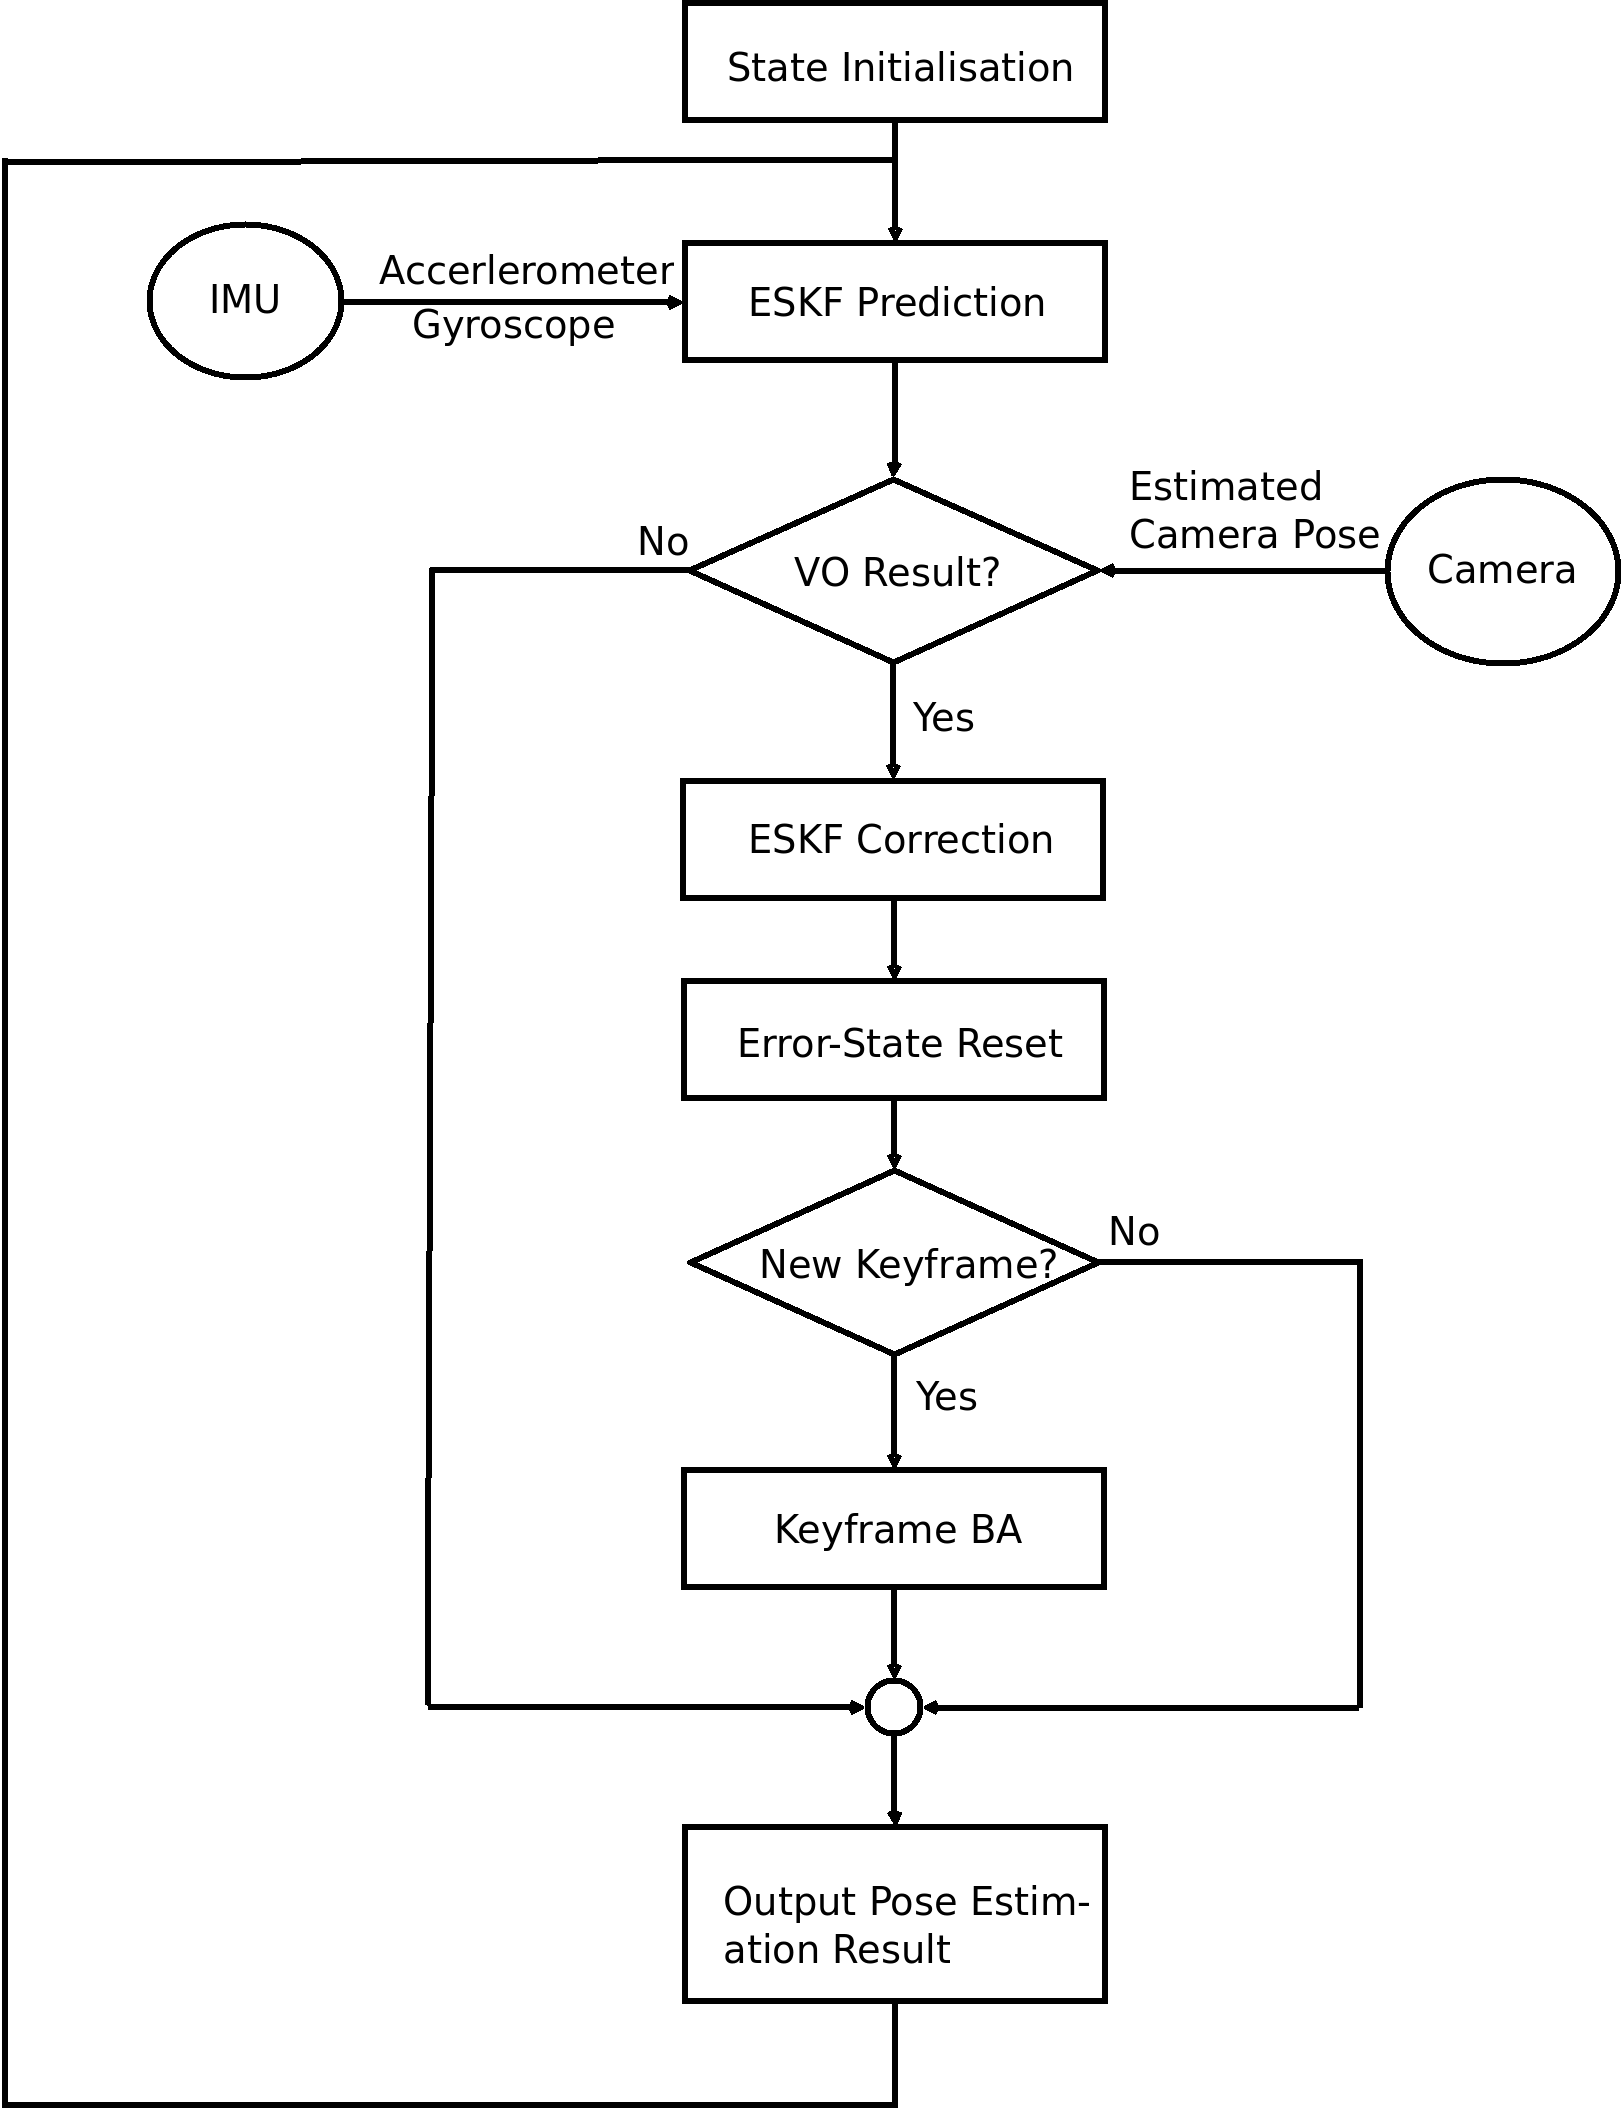
\includegraphics[width=0.5\textwidth]{CONTENT/Figure/Figure4-1_Pipeline.png}
    \caption{Pipeline of our visual-inertial odometry. Noted that measurement frequency from camera is 4 times lower than measurement frequency of IMU sensor in our experiment setting, therefore we do not have visual odometry (VO) result in some certain turn. Also whether this frame is keyframe is provided by VO.}
    \label{fig:fig4-1}
\end{figure}


In this section we summarize our visual-inertial odometry pipeline (see Figure \ref{fig:fig4-1}). We also analyses the computational cost of our visual inertial odometry system in this section.

An initialisation step is necessary for both nominal state and error state. After the system obtains measurements (\eg, 3-vector from accelerometer, and 3-vector from gyroscope) from IMU sensor, nominal state and error state are then predicted using Equation (\ref{f12}) to (\ref{f8}), and the system updates corresponding covariance matrix using Equation (\ref{f30}). 

If camera gives estimated camera pose in this turn, the system applies a \textit{correction step} as we have described in Section \ref{subsec:ESKF_IMU_sub4}. After injecting error state from nominal state, we obtain the estimated true state which contains camera pose. System then reset the error state, and further improving the odometry estimation quality by applying a keyframe bundle adjustment (keyframe BA) if this camera frame is specified as key frame by visual odometry as we have discussed in Section \ref{subsec:camera_comple_data_sub3}. Finally system output the estimated camera pose and starts the next round after receiving IMU measurements.

In our ESKF framework, computational complexity remains constant since we only keep the current states and covariance, and the size of states and covariance matrix are fixed during estimation process. To certify, we design an experiment (see Section \ref{subsec:experiment1}) to show that computational time remains unchanged when running a single IMU integration process using ESKF. As we discuss in Section \ref{sec:FVK}, the computational complexity is 
\begin{equation}
	O(m^2 \cdot n),
\end{equation}
where $m$ is the number of key frame, and $n$ is the number of landmarks. We claim that our odometry can also be extended to large scale since the number of landmarks can be enlarged and this in general is the key factor of limiting the scalability of SLAM-like system. Moreover it is also more beneficial to obtain high estimation accuracy by increasing the number of landmarks than number of key frames \cite{strasdat2010real}.

We are not able to build a environment map due to the time limitation of this master thesis. Although a few more map optimization steps are needed, the key frame BA we propose in Section \ref{subsec:camera_comple_data_sub3} gives a direct result of optimized landmarks, which are the main components of mapping. We explore this in future work chapter (Chapter \ref{chap:summary}).

All together, in this chapter we suggest an error-state Kalman filter (ESKF) based visual-inertial odometry. The system accurately estimates the camera-IMU platform pose by fusing the measurements from IMU and camera sensors. By using a loosely-coupled approach, system runs ESKF in a constant computational complexity and needs no special initialization steps, therefore it is suitable for localization of mobile robot in real-time. This odometry can also be extended to the large scaled scene, and/or an efficient SLAM system.

